\documentclass{article}

% Language setting
% Replace `english' with e.g. `spanish' to change the document language
\usepackage[english]{babel}

% Set page size and margins
% Replace `letterpaper' with `a4paper' for UK/EU standard size
\usepackage[letterpaper,top=2cm,bottom=2cm,left=4cm,right=4cm,marginparwidth=2.5cm]{geometry}

% Useful packages
\usepackage{amsmath}
\usepackage{graphicx}
\usepackage[colorlinks=true, allcolors=blue]{hyperref}

\title{CS307 Database project part2}
\author{Name: Wen Yinan\\
StudentID: 12310841\\
\vspace{1em} % 插入空行
Class#: Lab Mon 9-10\\
Name: Cui Zixuan\\
StudentID: 12311007\\
Class#: Lab Mon 9-10
}

\begin{document}
\doublespacing
\maketitle
\newpage
\tableofcontents

\newpage
\section{Information and Contribution}
\subsection{Contribution}

The basic information and contribution of our members are as follow.\\
- Cui Zixuan:
\begin{itemize}
    \item the basic backend implementation
    \item the implementation of the bonus method
    \item code optimization
    \item the completion of a small portion of the report
\end{itemize}
- Wen Yinan:
\begin{itemize}
    \item Connect the frontened and the complete backend system
    \item Construct the frontened web pages
    \item Design user's privilege. Realised login, logout, and admin management functions.
    \item ProjectReports
\end{itemize}

\subsection{Language}

We applied the following languages in our design\\
    Java 19.0.1 2022-10-18\\
    Java(TM) SE Runtime Environment (build 19.0.1+10-21)\\
    Java HotSpot(TM) 64-Bit Server VM (build 19.0.1+10-21, mixed mode, sharing)\\

\subsection{Test Environment}
We deployed two machines in our test\\
• HUAWEI SOUND(Processor: 13th Gen Intel(R)Core(TM)i5-13500H 2.60 GHz)\\
 • Lenovo Legion R9000x-2021-R(Processor: AMD Ryzen 7 5800H with Radeon Graphics            3.20 GHz)
\section{Database Design}
\subsection{Designing the E-R Diagram}
\subsubsection{ER Diagram Snapshot}
Below is a snapshot of the ER diagram we designed for our website:

\begin{figure}[h]
\centering % 确保图片居中显示
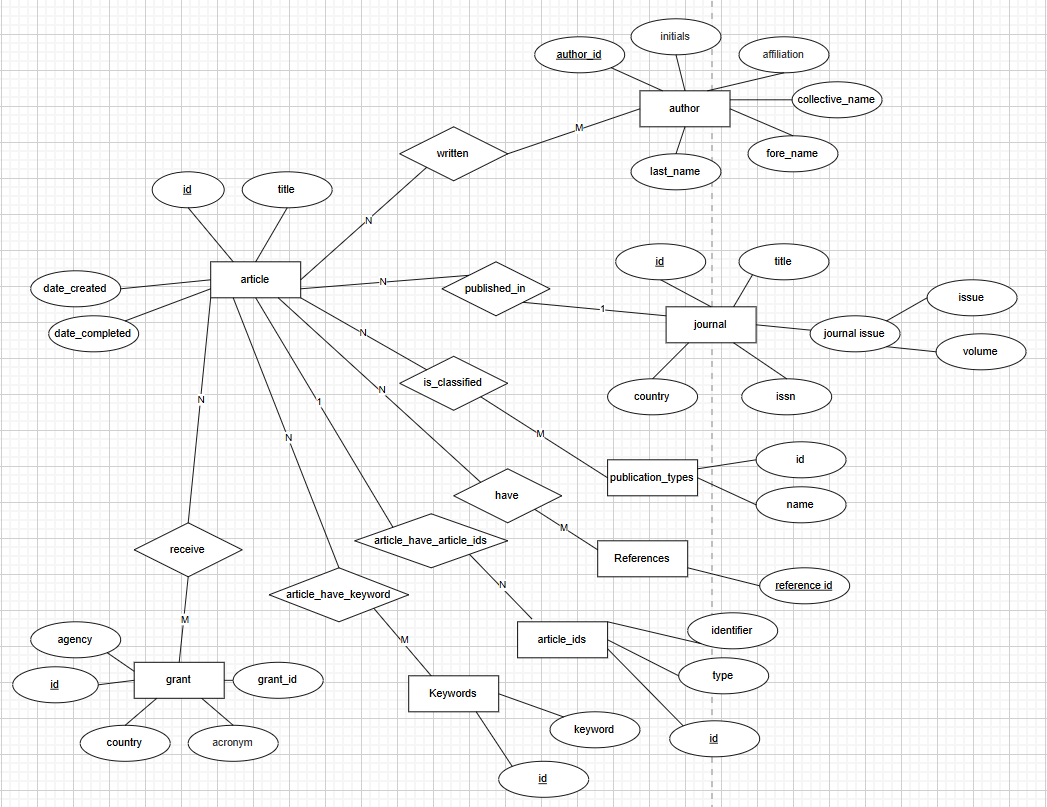
\includegraphics[width=.8\textwidth]{poject2ER.png} % 插入图片并调整大小
\caption{ER Diagram} % 为图片添加描述性标题
\label{fig:引用标签} % 为图片分配一个引用标签,方便后续引用
\end{figure}
 

This ER diagram provides a comprehensive view of the structure of the
database and how entities and attributes are interconnected.
\newpage
\subsection{Brief description}
\subsubsection{Tables and Columns}
Here is the database diagram for a clearer understanding of our database design.\\
% \newpage
\begin{figure}[h]
\centering % 确保图片居中显示
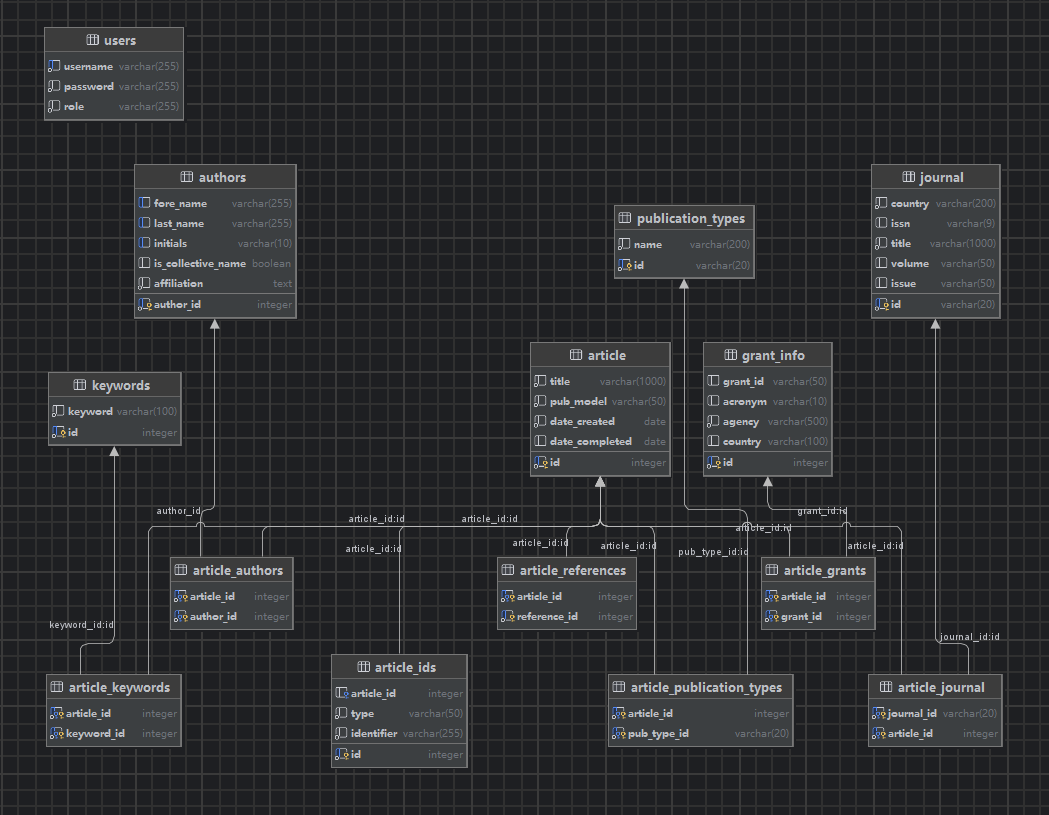
\includegraphics[width=.8\textwidth]{logic.png} % 插入图片并调整大小
\caption{database Diagram} % 为图片添加描述性标题
\label{fig:引用标签} % 为图片分配一个引用标签,方便后续引用
\end{figure}
We adjust the given "Goodloader" and add a user table to construct our database.
\newpage
\begin{itemize}
\item \textbf{Article Main Table}
\begin{enumerate}
\item \textbf{id(int, PRIMARY KEY, unique)}
\item \textbf{title(varchar(2550),not null):} We used the varchar(2550) data type for "title" to ensure it can accommodate sufficiently long article titles
\item \textbf{pub model(varchar(30))not null:} We utilized the varchar data type for ”pub model” as there are only five possible values for it : "Print" , "Print-Electronic" , "Electronic" , "Electronic Print" , "Electronic-eCollection".
\item \textbf{date created(date, not null):} We use the date data type for the DATE type ensures that date data is stored in a uniform format (YYYY-MM-DD), avoiding errors caused by inconsistent formats. Also by using the DATE type, the stored dates can be limited to a reasonable range, preventing the input of invalid dates such as "2024-13-01". Moreover, Using the DATE type can reduce unnecessary storage space usage, especially when dealing with large amounts of date data.
\item \textbf{date completed(date):} It is very similiar to the colume "date created".

\end{enumerate}

\item \textbf{Authors Main Table}
\begin{enumerate}
\item \textbf{author id(serial PRIMARY KEY):} We choose serial as its datatype to create a unique primary key. It ensures each relationship
has a unique identifier, and the identifier increments automatically, making it easy to manage.
\item \textbf{lastname(varchar(255))}
\item \textbf{forename(varchar(255))}
\item \textbf{initials(varchar(10))}
\item\textbf{affiliation(text)}
\item \textbf{is collective name(boolean)}  
\end{enumerate}


\item \textbf{Journal Main Table}
\begin{enumerate}
\item \textbf{journal id(varchar(40) PRIMARY KEY}
\item \textbf{title(varchar(2550),not null)}
\item \textbf{country(varchar(100))}
\item \textbf{issn(varchar(20))}
\item \textbf{journal-issue-issue(varchar(200))}
\item \textbf{journal-issue-volume(varchar(200))}
\end{enumerate}


\item \textbf{Grant info Main Table}
\begin{enumerate}
\item \textbf{grant id(varchar(50) PRIMARY KEY):}
\item \textbf{agency(varchar(255) not null):} We used the varchar(255) data type for ”agency” to ensure it can accommodate sufficiently long agency name.
\item \textbf{country(varchar(70))}
\item \textbf{acronym(varchar(50))}
\end{enumerate}

\item \textbf{Article Ids Main Table}
\begin{enumerate}
\item \textbf{article id(int)}
\item \textbf{id(int PRIMARY KEY)}
\item \textbf{type(varchar(10) PRIMARY KEY)}
\item \textbf{identifier (VARCHAR(255) NOT NULL)}
\end{enumerate}

\item \textbf{Publication Types Main Table}
\begin{enumerate}
\item \textbf{publication type id(varchar(50) PRIMARY KEY):}
\item \textbf{name(varchar(50))}
\end{enumerate}


\item \textbf{keywords Main Table}
\begin{enumerate}
\item \textbf{id(int PRIMARY KEY):}
\item \textbf{keyword(varchar(100))}
\end{enumerate}


\item \textbf{User Main Table}
\begin{enumerate}
\item \textbf{username(varchar(255) PRIMARY KEY):} 
\item \textbf{reference id(varchar(255),PRIMARY KEY)}
\item \textbf{role (varchar(255),PRIMARY KEY)}It must be user or admin
\end{enumerate}

\end{itemize}
\end{itemize}
\begin{itemize}
\item \textbf{article-authors Table,article-publication-type Table,article-grants Table,article-references Table,article-journal Table,article-keywords Table:} This six tables share similar structures, aiming to connect the article with author, article with publication type, and article with grant by their id.
\begin{enumerate}
\item \textbf{article id(int PRIMARY KEY)}
\item \textbf{author/publication type/grant id(int PRIMARY KEY)}
\end{enumerate}

\end{itemize}
\subsubsection{Privilege}
We divided users into "user" and "admin". Users can only reach functions of seaching such as getArticleCitationsByYear, getArticlesByAuthorSortedByCitations, getJournalWithMostArticlesByAuthor, getMinArticlesToLinkAuthors, getCountryFundPapers, getImpactFactor, getArticleCountByKeywordInPastYears

Whenever a account is added, we will add the new information into the table "User". Also, we enables admins to delete users in the table to better manage the database.
\begin{figure}[h]
\centering % 确保图片居中显示
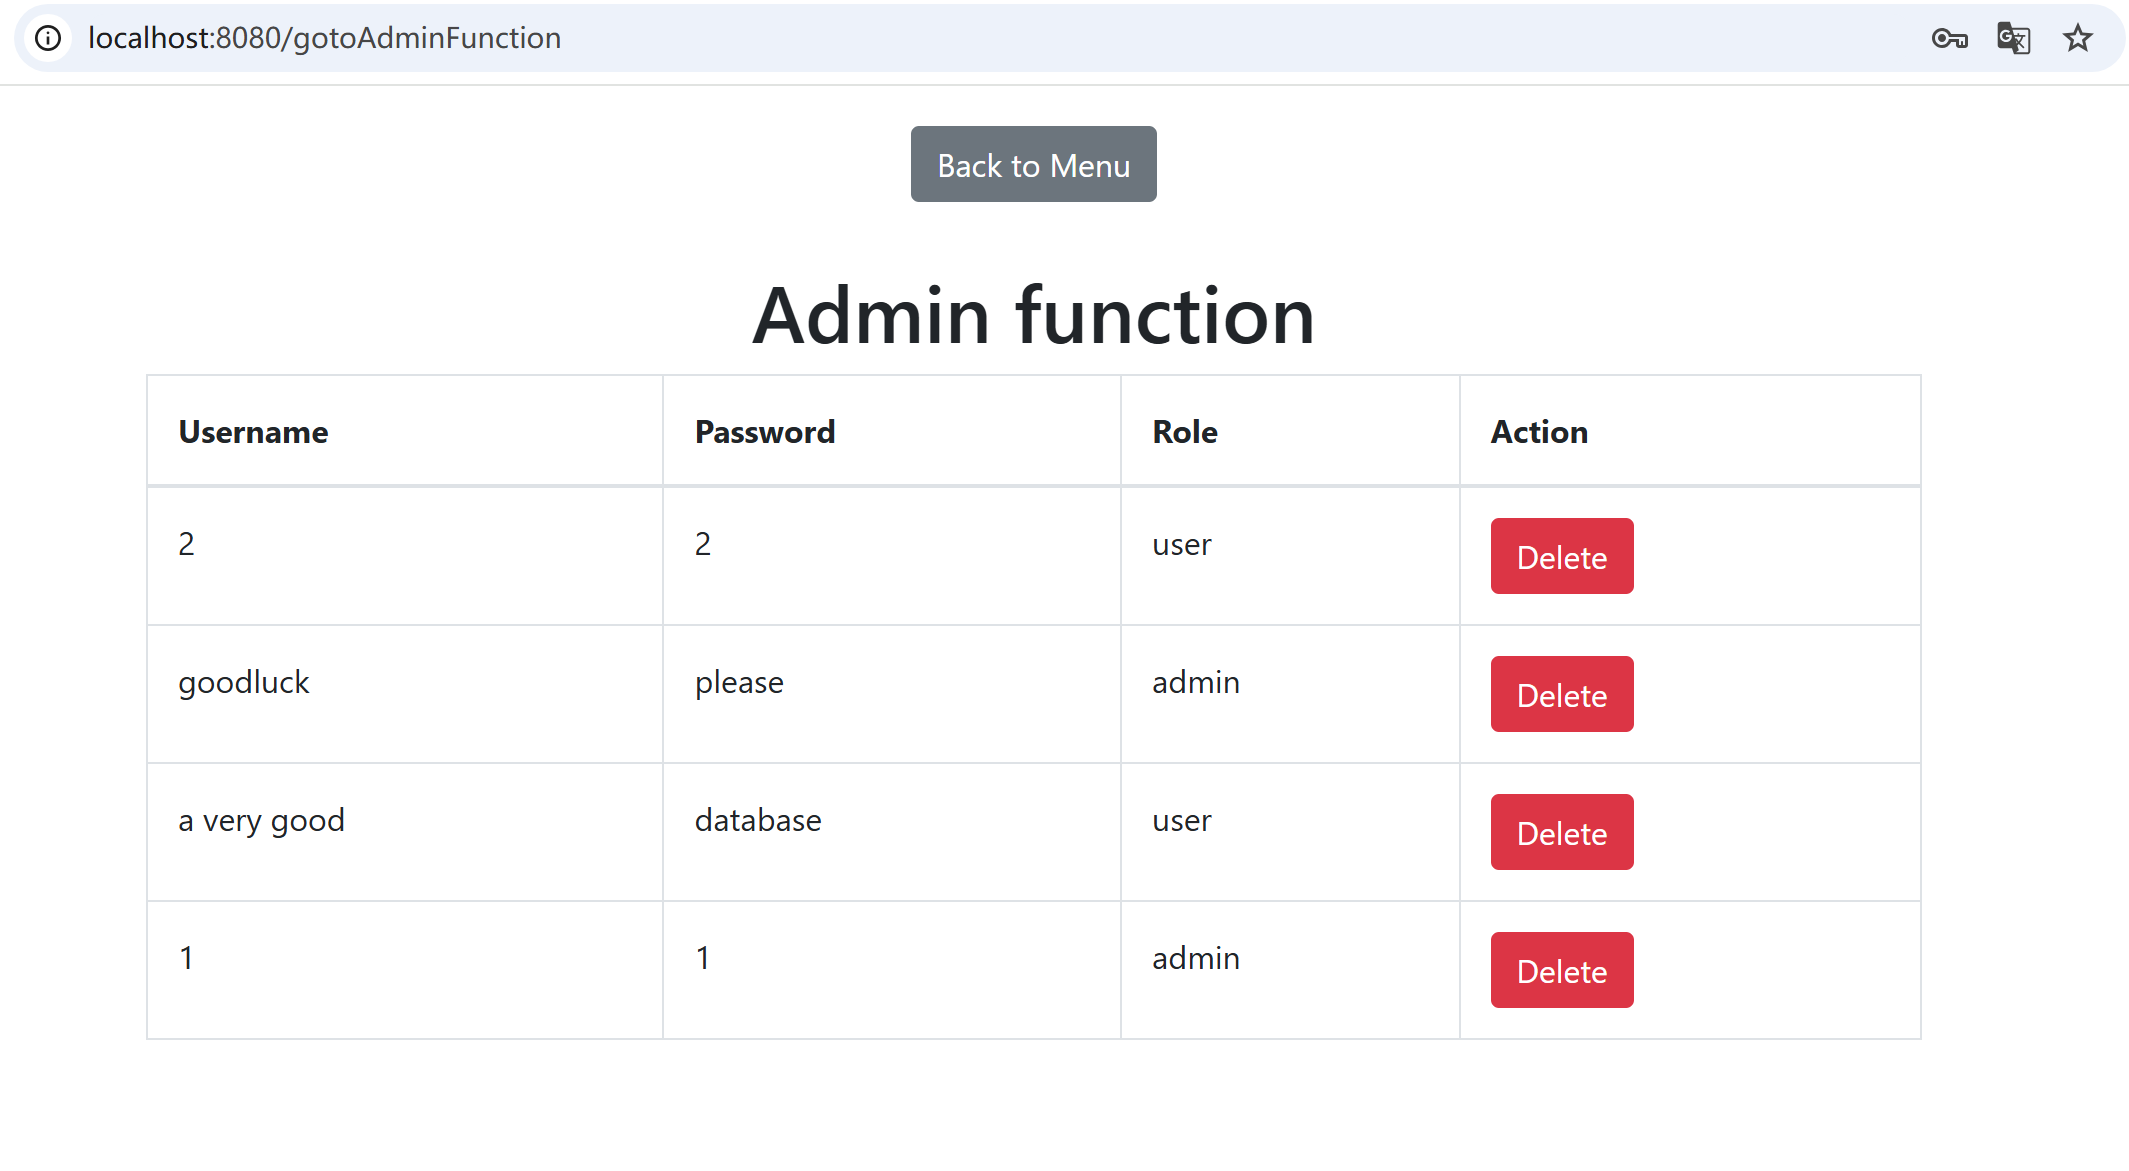
\includegraphics[width=.8\textwidth]{权限.png} % 插入图片并调整大小
\caption{admin priviledge} % 为图片添加描述性标题
\label{fig:引用标签} % 为图片分配一个引用标签,方便后续引用
\end{figure}

\section{Basic API Specification}
\subsection{Raw Data}
The data file is pubmed24n.ndjson
\subsection{Implementation Techniques}
In this section, we outline the key techniques used in implementing the back-end functionalities, with a focus on dynamic SQL execution, error handling, and performance optimization.


\subsubsection*{\uppercase\expandafter{\romannumeral+1} Temp Table for Citation Count}
To improve performance in handling APIs related to article citations, we created a temporary table to store the citation count for each article. This optimization eliminates the need for repeated computations during API requests. Key steps include:
\begin{itemize}
    \item Populating the temp table during the initial data import phase.
    \item Maintaining data correctness during article updates and deletions.
    \item Leveraging indexing on the temp table for faster query execution.
\end{itemize}

\subsubsection*{\uppercase\expandafter{\romannumeral+2} Dynamic SQL Statements}
We utilized dynamic SQL statements, dynamically adjusting the update SQL queries based on data received from the front-end. This approach ensures flexibility and efficiency, allowing different SQL queries to be constructed based on varying data conditions.

\subsubsection*{\uppercase\expandafter{\romannumeral+3} Error Handling and Logging}
Robust error handling mechanisms were employed to ensure API stability:
\begin{itemize}
    \item Catching and gracefully handling all exceptions without propagating them to the API layer.
    \item Logging errors with sufficient details for debugging using the SLF4J logging framework.
    \item We created a dedicated \texttt{LogManager} class to manage error handling and logging, making it easier to view and manage log information.
\end{itemize}

\subsubsection*{\uppercase\expandafter{\romannumeral+4} Bonus Methods}
 
We adopted a BFS approach combined with a materialized view. The materialized view serves as an intermediate table, enabling us to efficiently query information about articles, including their references and the articles that reference them. This setup significantly accelerates the query process to some extent.
Additionally, the core algorithm involves a standard BFS procedure. 
Moreover, we implemented a class named MaterializedViewRefresher, which updates the materialized view in response to changes in the underlying tables, ensuring the view remains up-to-date through a refresh mechanism.

This systematic approach ensures a robust, maintainable, and high-performance back-end system.






\section{Advanced APIs and Other Requirements}
In this part, we developed a web application using Spring Boot for the backend and Thymeleaf for the frontend to handle user interactions and manage functionalities such as login, logout,  permission control,and the above 9 APIs.


\subsection{Backend (Spring Boot)}
\subsubsection{Controller Layer}
\begin{itemize}
    \item{In Spring Boot, We created Controller classes annotated with @Controller to handle HTTP requests. Each controller method corresponds to an endpoint that performs specific actions like user registration, login, and logout. For example, the UserController handles user-related operations.}
    \item{The methods in the controller use annotations like @GetMapping and @PostMapping to map specific HTTP methods (GET, POST) to the corresponding actions.}
    \item{For example, the /login endpoint accepts the username and password from the frontend, checks the credentials via the service layer, and then decides the response (either login failure or redirect to a homepage).}
\end{itemize}

\subsubsection{Service Layer}
\begin{enumerate}
\item Open your Datagrip and click the File option and you will find a new option, make your mouse hanging on the New option and you will will find a DataSource option in the new line showned.
\item Click the DataSource option and choose the PostgresSQL option and click.
\item In the new window named DataSource and divers, edit the username and your password to finish the last step.
\item Click the Test Connection button to ensure you have down load the necessary diver.
\item Open our IDEA java codes and enter the Main class, change the file path into yours. And enter the Datamanager class just change the URL, Username, and the password.
\item Till now, you can cilick the Main button and run the codes to import Data!!!
\end{enumerate}
\subsubsection{Model and Data Binding}
\begin{itemize}
    \item{The data from the controller is passed to the frontend via the Model object, which stores the attributes that will be rendered by Thymeleaf. For instance, in the login process, user data or error messages are added to the model (model.addAttribute("error", "Invalid username or password")).}
    \item{Spring Boot uses ModelAndView to send the data and specify the view name (i.e., the Thymeleaf template) to be rendered.}
\end{itemize}
\subsection{Frontend (Thymeleaf)}
\subsubsection{Thymeleaf Templates}
\begin{itemize}
    \item{Thymeleaf templates (HTML files) are stored in the src/main/resources/templates/ directory. These templates contain the HTML structure of the page along with Thymeleaf-specific syntax for data binding.}
    \item{We use Thymeleaf expressions (e.g., ${error}, ${username}) to insert dynamic data from the controller into the HTML.}
\end{itemize}

\subsubsection{Dynamic Content Rendering}

Thymeleaf tags are used for rendering dynamic content. For example, th:text is used to insert text, and th:if is used to conditionally display elements. This is particularly useful when displaying messages like login errors or the user's name.
\subsubsection{Form Handling}
We used the <form> tag in Thymeleaf to handle user inputs and bind them to the backend. For instance, the login form in login.html binds the username and password fields to the corresponding parameters in the controller method using th:field.


\section{Conclusion}
In this project, we implemented a robust and scalable backend system using Spring Boot, PostgreSQL, and Thymeleaf to meet the requirements for handling article data, user interactions, and permissions. By incorporating optimization techniques such as the use of temporary tables for citation counts and dynamic SQL statements, we enhanced the performance and flexibility of the system, ensuring that it could handle complex queries and data updates efficiently.

The implementation of dynamic SQL allowed us to handle varying data conditions dynamically, making the system adaptable to different use cases. Meanwhile, the use of materialized views and recursive SQL queries provided significant performance improvements by storing precomputed results and refreshing them periodically through scheduled tasks.

Error handling and logging were carefully integrated into the system, ensuring that all exceptions were caught and logged for easy debugging. The integration of SLF4J logging and a dedicated LogManager class further streamlined the process of managing and analyzing logs.

On the frontend, Thymeleaf templates were employed to create dynamic, user-friendly interfaces that bind seamlessly with the backend. Through careful use of dynamic content rendering and form handling, we ensured that the user experience was smooth and interactive, with clear messages and form data binding for actions like login and registration.

Overall, this approach resulted in a robust, maintainable, and high-performance backend system that meets the needs of both data handling and user interaction, while also being flexible enough to accommodate future growth and improvements.






% \subsection{How to add Lists}

% You can make lists with automatic numbering \dots

% \begin{enumerate}
% \item Like this,
% \item and like this.
% \end{enumerate}
% \dots or bullet points \dots
% \begin{itemize}
% \item Like this,
% \item and like this.
% \end{itemize}





\end{document}